\documentclass[11pt]{article}
\usepackage[margin=1in]{geometry}
\usepackage[T1]{fontenc}
\usepackage[utf8]{inputenc}
\usepackage{lmodern}
\usepackage{microtype}
\usepackage{graphicx}
\usepackage{booktabs}
\usepackage{array}
\usepackage{amsmath}
\usepackage[hidelinks]{hyperref}
\hypersetup{
  pdftitle={Held-out value copying in small language models: a field-localized failure mode and the instrument to measure it},
  pdfauthor={Hassan El Jesr}
}
\usepackage[round]{natbib}
\graphicspath{{../figures/}}

\title{Held-out value copying in small language models:\\ a field-localized failure mode and the instrument to measure it}
\author{Hassan El Jesr\\ \texttt{summer.say3y@icloud.com}}
\date{July 2026}

\begin{document}
%% Camera-ready sync from papers/paper1_draft.md (scope lock 2026-07-31).
%% Measurement-only Paper~$\alpha$. E1 KILL recorded. No architecture/product thesis.

\maketitle

\begin{quote}
\small
\textbf{SRC baseline (2026-07-30; scope lock 2026-07-31):}
this manuscript is \textbf{Paper~$\alpha$ --- measurement only}.
Surviving contribution: under low-diversity extraction regimes, small transformers can converge to closed-set prediction strategies that fail held-out symbolic emission; diversity and adaptation regime change the measured reliability profile.
\textbf{Not} an architecture or product thesis; \textbf{not} a claim that generative LM + verify is the right substrate.
Mechanism language in related-work is hypothesis framing only.
Systems/verification claims (if any) are out of scope here.
See \texttt{papers/EMPIRICAL\_FOUNDATION.md}.
\end{quote}

\begin{abstract}
We study a specific faithfulness failure in small language models finetuned to convert short clinical dialogues into structured summaries: a \textbf{held-out copying gap} --- the model copies field values it saw during finetuning but errs on held-out values under held-out phrasings, even though both are present verbatim in the input. In our own from-scratch models (3.15M and 10M parameters) this gap is large --- $18.3\pm1.3$ and $18.7\pm1.5$ points of recall on the same multi-instance instrument used for the rest of the ladder (22--23 points on the single public instance the anchors were first scored on; \S\ref{sec:ladder}). The failure is not diffuse: it localizes \emph{entirely} to the three open-vocabulary fields (complaint, medication, allergy) and is \textbf{exactly zero} in the two closed-value fields (duration, severity), which act as a built-in control showing the effect is specifically held-out-\emph{value} copying in open slots, not a generic degradation under unfamiliar phrasing. Finetuning the Pythia open-weight family (160M/410M/1B) on the identical task, the gap observed is \textbf{substantially smaller} (single-digit points; 3.5$\pm$0.7 at 160M, 4.2$\pm$0.9 at 410M, and an interval of $[0,5]$ at 1B) --- and that residual is itself field-localized: per-field re-scoring shows Pythia fully solves held-out complaints and medications, while its entire remaining gap is the one open slot with only five training values (allergy), where even 410M fails totally on the held-out value. We deliberately do \textbf{not} claim scale as the cause: the comparison also changes pretraining corpus, tokenizer, architecture, and finetuning method. A within-stack control at $\sim$160M keeps that stack fixed and finds the diluted gap still $16.9\pm1.7$ under full FT on $\sim$200M pretraining tokens. Across the evaluated own-stack configurations, the held-value copying gap did not decrease monotonically with parameter count. Parameter count was not isolated from total pretraining exposure (3.15M used \textbf{32.8M} tokens; 10M and the weak 160M cell used $\sim$\textbf{200M}; the Chinchilla 160M cell used \textbf{3.2B}), so this result is descriptive and does not establish a parameter-only scale law. LoRA or Chinchilla-scale data each reduce the diluted gap to $\sim$7 and both together to $4.2\pm0.9$ --- an adaptation$\times$data \textbf{interaction}, not a pure scale law. Separately, a pre-registered slot-diversity sweep lifts held-type recall on that open slot by \textbf{+66.7} points (D5$\rightarrow$D80) at fixed scale. On a pre-registered utility, the generator-aligned non-generative baseline \textbf{M1} scored $0.998999$ and exceeded the best evaluated generative reference, official M0 at $0.925217$ (\S\ref{sec:e1}; \textbf{KILL}); this paper reports that result honestly and does not advocate a generative substrate. Primary metrics are exact string match; dual-clinician / human-accepted equivalence is unvalidated (\S\ref{sec:e1}, \S\ref{sec:limitations}; a bounded agent-applied rubric audit is reported there). Measurement reliability is a second contribution: single-instance evaluation was under-powered, and at 1B \textbf{training-run nondeterminism} dominates the residual. Both lessons arose from empirical failures of the prior instrument, not from foresight.
\end{abstract}

% Locked draft places E1 at §0 (kill-gate before Introduction).
\setcounter{section}{-1}
\section{Non-generative baseline M1 exceeds generative references under frozen $U$ (E1; locked)}\label{sec:e1}

On the pre-registered utility $U = P - 0.5\,M - 0.3\,\rho - 0.02\,L - 0.05\,C$ with decision margin $\delta=0.05$, scored methods include official generative LM references on RunPod CUDA fp16 (frozen recipes) and classical/constrained baselines on the same harness (\texttt{trajectory/results\_e1\_utility.json}):

 \begin{center}
\begin{tabular}{ll}
\toprule
Method & $U$ (verify-on) \\
\midrule
M1 template / rules & 0.999 \\
Official M0 (Pythia-160M LoRA) & \textbf{0.925} \\
Own-stack Chinchilla + LoRA & 0.898 \\
M2 dict + span & 0.886 \\
Local M0 (scale-10M) & 0.854 \\
\bottomrule
\end{tabular}
\end{center}

\textbf{Verdict: KILL (H-substrate).} Under frozen $U$, the generator-aligned non-generative baseline \textbf{M1} scored $0.998999$ and exceeded the best evaluated generative reference, official M0 at $0.925217$. M2 ($U\approx0.886$) does \textbf{not} meet the registered dominance criterion versus official M0 (it is within $\delta=0.05$ but does not beat it). Sensitivity did not flip the M1 kill. Paper~$\alpha$ therefore continues strictly as \textbf{measurement} of when small LMs fail held-out emission --- not as advocacy for a generative substrate. A different utility could re-rank methods; the field-localization / diversity / scaling measurements do not depend on $U$.

\textbf{Exact-match construct limitation.} Primary science metrics use exact string match on field values. Automated normalize-then-match does not rescue M0 exact failures (0/486; \texttt{trajectory/results\_e3\_normalize\_construct.json}). A bounded \textbf{agent-applied rubric audit} of 100 sampled errors (\texttt{trajectory/results\_e3\_human.json}, rater \texttt{agent-rubric-pass-1}) classified \textbf{0/100} as acceptable semantic equivalents. This result does \textbf{not} substitute for independent clinician annotation, inter-rater agreement, or validation of a synonym ontology. Reported gaps may overstate failure relative to a soft/human rubric. This is an explicit limitation of Paper~$\alpha$. No open-world verification claims are made here.

\textbf{Out of scope here:} LoRA mechanism (unidentified); E2/fabric/product claims; token-coverage effect sizes beyond description; open-world verifier guarantees.

\section{Introduction}\label{sec:intro}

Structured summarization is often judged not on average-case benchmark scores but on faithfulness under distribution shift: whether the output contains only content grounded in the input, including on inputs unlike the training data (Maynez et al. 2020; {Ji et al.} 2023). We isolate one tractable component of this --- value copying --- in a synthetic structured-summarization task where faithfulness is measurable by construction, and ask a single pre-registered question: \textbf{how does the copying gap behave as model capability increases?}

The contribution is measurement-only and we keep the parts distinct: 1. \textbf{Empirical core.} Field-localized held-out copying failure in small models; descriptive own-stack scale/config comparison and base$\times$method interaction (\S\ref{sec:withinstack}); causal slot-diversity effect (+66.7; \S\ref{sec:diversity}); residual floor on the hardest low-diversity open slot (\S\ref{sec:withinstack}). 2. \textbf{Measurement lessons.} Single-instance evaluation was under-powered (\S\ref{sec:underpowered}); training nondeterminism bounds the top rung (\S\ref{sec:nondet}); exact-match is an explicit construct limitation (\S\ref{sec:e1}, \S\ref{sec:limitations}). 3. \textbf{Substrate note (\S\ref{sec:e1}).} Under a pre-registered utility, \textbf{M1} exceeds the best evaluated generative reference on this task (\textbf{KILL}). Recorded honestly; not a product or architecture claim.

\section{Related work}\label{sec:related}

\emph{Citations verified against primary sources (§ References). Framed only as context for the measured copying gap and evaluation reliability --- not as architecture or substrate advocacy.}

\textbf{Scaling laws and emergence.} Language-model loss follows smooth power laws in parameters, data, and compute ({Kaplan et al.} 2020; {Hoffmann et al.} 2022), yet specific \emph{task} behaviors can change sharply with scale: {Wei et al.} (2022) catalogue ``emergent abilities'' absent in small models and present in large ones. Schaeffer et al. (2023) argue much apparent emergence is a \emph{measurement artifact} of discontinuous metrics (exact-match, multiple-choice) rather than a property of the model. Our study runs in the opposite direction --- a behavior (the held-out copying gap) that is \emph{large} in small models and \emph{smaller} at larger scale --- but Schaeffer et al.'s caution applies directly, since our gap is an exact-match recall difference; we therefore report it with across-instance error bars and, at 1B, separate metric behavior from training-run variance (\S\ref{sec:nondet}). Where the emergence literature asks ``does scale switch an ability \emph{on}?'', we ask ``does scale switch a faithfulness failure \emph{off}?'', and find the honest answer is confounded with the training stack (\S\ref{sec:limitations}).

\textbf{The Pythia platform.} {Biderman et al.} (2023) release Pythia, 16 models spanning 70M--12B trained on identical data in identical order, expressly to make scale a controlled variable. We use the 160M/410M/1B rungs as our scaling axis for exactly this property --- within Pythia, architecture, tokenizer, pretraining corpus, and data order are fixed across sizes. The limitation we foreground (\S\ref{sec:limitations}) is that our own-stack anchors are \emph{not} in that controlled family, so the nano$\rightarrow$Pythia step moves the stack as well as the scale --- a confound Pythia's internal control cannot remove.

\textbf{Copying behavior (context only).} The behavior we measure is value \emph{copying}: reproducing a field value present verbatim in the input. Prior seq2seq copy modules (CopyNet (Gu et al. 2016); pointer-generator (See et al. 2017) and transformer copy/retrieval hypotheses ({Elhage et al.} 2021; {Olsson et al.} 2022; Wu et al. 2024) are cited only as background for \emph{what was measured}. This paper does not identify circuits, compare substrates for product choice, or claim a generative architecture is preferable; mechanism work remains gated (\texttt{papers/EMPIRICAL\_FOUNDATION.md}).

\textbf{Faithfulness and hallucination.} Faithfulness --- output grounded only in the input --- is a central failure mode of abstractive summarization; Maynez et al.~(2020) distinguish intrinsic (misrepresenting source content) from extrinsic (unsupported) hallucination, and Ji et al.~(2023) survey the phenomenon across NLG. Most such work relies on human judgment or model-based entailment scoring. Our task is constructed so faithfulness is \emph{exact}: because each dialogue is rendered from a known fact tuple, a summary is scored field-by-field against ground truth with no judge model, and our ``hallucination'' is precisely an extrinsic fabrication of a field value. This trades ecological realism for a noise-free, reproducible faithfulness signal.

\textbf{Reproducibility and training nondeterminism.} Run-to-run variation from seeds and low-level tooling can be large enough to reverse method rankings (Picard 2021; Pham et al. 2020), and even fixed-seed training is nondeterministic through non-associative GPU reductions and library tooling (Zhuang et al. 2022); the standard prescription is to report mean $\pm$ SD over multiple runs. Our 1B result is a concrete downstream instance: two fixed-seed retrains of the same model produced gaps of 5 and 0 on the byte-identical evaluation, so at that rung the \emph{unit of uncertainty} shifts from the evaluation instance to the training run, and we report an interval (\S\ref{sec:nondet}). This connects the reproducibility literature to a specific measured behavior (a faithfulness gap) rather than to top-line accuracy.

\textbf{Evaluation reliability and contamination.} Public benchmarks risk contamination --- memorized test content inflating scores (Xu et al. 2024) --- with held-out or rolling test data the standard defense. Our benchmark is a \emph{seeded generator} rather than a fixed set, so fresh evaluation instances can be drawn at will, and our pre-registered contamination check compares the public instance against fresh draws. We find the public instance is \emph{harder} (higher gap) than fresh draws at every rung --- the opposite of the contamination signature --- which both rules out memorization and surfaces a distinct hazard: a fixed public instance can be a systematically biased difficulty draw even when content-addressed and reproducible.

\section{Task and benchmark}\label{sec:task}

\emph{This section motivates the design; the precise protocol (generator, held-out split, metric) is in Methods.}

\textbf{Faithfulness is exact by construction.} Synthetic clinic dialogues are rendered from a known fact tuple of five fields (chief complaint, duration, severity, medication, allergy), so each summary is scored field-by-field against ground truth with no judge model --- a noise-free faithfulness signal, traded against ecological realism.

\textbf{The held-out copying gap.} Evaluation dialogues are held-out along two axes --- held-out \emph{template families} (all dialogues) and held-out \emph{slot values} (half the dialogues) --- and the central object is the \textbf{held-out copying gap}: seen-value recall minus held-out-value recall under held-out templates, which isolates value copying from phrasing familiarity.

\textbf{The benchmark is a generator.} The scientific object is the eval \emph{distribution} (a seeded generator), not any fixed set of dialogues. Fresh instances can be drawn to defend against memorization of any specific instance (\S\ref{sec:underpowered}), and the instance-difficulty distribution can be measured directly --- a property we exploit in both measurement lessons.

\section{Prior stages (setup)}\label{sec:prior}

Two earlier results frame the question. \textbf{Stage C} tested whether the gap is a training-curriculum artifact by adding an unmemorizable-value training slice; the held-out gap was unmoved, refuting the curriculum explanation. \textbf{Stage S} scaled our own stack from 3.15M to 10M parameters: the larger model passed the average-case faithfulness gate (parse 100\%, recall 88\%, hallucination 7.5\%) yet its held-out gap was essentially unchanged ($\approx$23 vs $\approx$22 points single-instance; $18.7\pm1.5$ vs $18.3\pm1.3$ on the multi-instance instrument, \S\ref{sec:ladder} --- the near-identity now measured with error bars, not two single points). Stage S concluded that a 3.2$\times$ scale step does not cross the failure --- motivating a wider ladder.

\section{Stage T design (pre-registered)}\label{sec:design}

\textbf{Ladder.} Own models at 3.15M/10M (re-scored on the multi-instance instrument, \S\ref{sec:ladder}) plus the Pythia family at 160M/410M/1B, finetuned on the identical scribe recipe with LoRA and scored by the identical faithfulness scorer (full configuration in \S\ref{sec:methods}).

\textbf{Why Pythia.} The question is scaling behavior, not model ranking. Pythia (Biderman et al., 2023) holds architecture, tokenizer, pretraining corpus, and data order fixed across sizes, so within the family relatively few variables move with parameter count --- the property a scaling study needs. This choice does not isolate scale from the nano$\rightarrow$Pythia \emph{stack} change (\S\ref{sec:limitations}); it is the reference family for that axis, not a claim that scale is the cause.

\textbf{Pre-registration and falsifiers.} Bars, bands (PERSISTS/THRESHOLD/DIVERGENT), seeds, and decision rules were fixed before measurement (\texttt{PREREG.md}, three pre-measurement amendments). A base-model control (un-finetuned model must fail parse \textless{} 50\%) guards against a trivially-solvable task; it passed at every rung (base parse 0\%). The measured code was adversarially reviewed before any run; three measurement-invalidating defects were fixed pre-measurement.

\section{The measurement instrument, and why it changed}\label{sec:instrument}

The instrument evolved because the data demanded it. We present this as a result.

\subsection{Single-instance evaluation was under-powered}\label{sec:underpowered}

The pre-registered contamination check (score the same model on the public instance vs.~a fresh instance; require per-metric agreement within 5 points) \textbf{flapped} at the threshold across rungs (gap differences $\approx$5, 6, 4). We attribute this to the gap riding on a handful of hard held tokens, so a single 20-dialogue instance carries $\pm$5--6 points of sampling variance. Crucially, the \emph{direction} of the discrepancy (the public instance was \textbf{harder}, not easier) is the opposite of the contamination signature the check was built to detect --- ruling out memorization. The fix (T-v2) re-scores the same frozen models on \textbf{five instances of 100 held dialogues each} and reports the gap as a mean $\pm$ across-instance SD. This cut the SD to $\sim$0.7--0.9 points at 160M/410M. We applied the identical re-scoring to the own-stack anchors so the whole ladder shares one instrument (\texttt{PREREG\_anchors.md}, re-scoring only --- frozen v0.1 checkpoints, their native ChatML/greedy scorer; both anchors reproduced their canonical single-instance readings byte-for-byte before the multi-instance pass). The anchors' single public-instance gaps (22.4, 23.0) were themselves modestly hard draws --- $\sim$4 points above their multi-instance means (18.3, 18.7) --- the \textbf{same direction} (public instance harder, not easier) found at the Pythia rungs, so the public instance is a systematically hard draw across the entire ladder.

\subsection{Training nondeterminism bounds the 1B estimate}\label{sec:nondet}

T-v2 re-generates each frozen adapter by re-finetuning at the fixed seed; we verify this reproduces the original model by re-scoring the byte-identical original instances and checking the gaps match (a \textbf{determinism cross-check}). At 160M and 410M the match was exact. At 1B it \textbf{failed}: on the byte-identical instance, one training run gave a 5-point gap and another gave 0. With evaluation held constant, the difference is training-run variance --- fp16 with non-associative GPU reductions over $\sim$1125 steps of a 1B model that, we conjecture, sits near the boundary of perfect held-out copying --- the tooling-level nondeterminism documented by Zhuang et al.~(2022) (cf.~Picard, 2021, on seed variance exceeding effect sizes), here surfacing in a downstream faithfulness metric rather than top-line accuracy. The right instrument for the 1B gap is therefore multiple training seeds, not multiple evaluation instances; we report an interval. With only two retrains we bound the \emph{magnitude} of training-run variance at this rung (it is large --- comparable to the whole residual gap) but cannot characterize its distribution; the interval spans the two observed outcomes rather than a modelled spread, and a fuller characterization (how often a run tips to perfect held-out copying) would need more seeds.

\subsection{Consolidated protocol}\label{sec:methods}

\emph{Authoritative protocol; \S\ref{sec:task}/\S\ref{sec:design}/\S\ref{sec:instrument} give motivation and instrument evolution. Every artifact below is content-addressed in \texttt{REPRODUCIBILITY.md}.}

\textbf{Datasets (a seeded generator).} Each example is a synthetic doctor--patient dialogue rendered from a fact tuple of five fields --- chief complaint (cc), duration (dur), severity (sev), medication (med), allergy (alg) --- paired with the target summary \texttt{CC:\ …\ \textbar{}\ DUR:\ …\ \textbar{}\ SEV:\ …\ \textbar{}\ MED:\ …\ \textbar{}\ ALG:\ …}. Training values (seen): a fixed complaint pool plus a compositional body-part$\times$sensation pool ($\sim$190 complaints, so cc cannot be solved as closed-set classification), 18 medications, 5 allergies, 3 severities. Finetuning data: 12,000 examples, full supervised finetune, 3 epochs, LR 1e-4 (own stack); the eval distribution is a separate v1 generator.

\textbf{Held-out protocol (two axes).} Evaluation dialogues are held-out along two independent axes. (i) \emph{Held template families}: doctor/patient surface phrasings never seen in finetuning --- used by \textbf{all} eval dialogues. (ii) \emph{Held slot values}: six specific values excluded from all finetuning data (complaints \{toothache, neck pain, heartburn\}, medications \{melatonin, throat lozenges\}, allergy \{sulfa drugs\}) --- used by \textbf{half} the eval dialogues; the other half draw seen values. The \textbf{held-out copying gap} = seen-value recall - held-out-value recall, both measured under held templates, isolating value copying from phrasing familiarity.

\textbf{Model families and finetuning.} \emph{Own stack}: from-scratch GPT (RoPE, GQA, SwiGLU, RMSNorm pre-norm, tied embeddings, 4098-vocab BPE, 512 ctx) at 3.15M (d=192, L=6, H=6, KV=2, ff=512; pretrained on \textbf{32.8M} FineWeb tokens over $\sim$3.1 epochs of a 10.96M-token shard; \texttt{pretrain/AUDIT.md}) and 10M (d=320, L=8, H=8, KV=2, ff=864; pretrained on $\sim$\textbf{200M} tokens, D$\approx$20N; \texttt{scale/AUDIT.md}; {Hoffmann et al.} 2022), full-FT on the scribe task; the two anchor checkpoints are the frozen v0.1 release assets (\texttt{scribe.pt}, \texttt{scale10m\_scribe.pt}). Later own-stack 160M configurations used approximately \textbf{200M} or \textbf{3.2B} pretraining tokens depending on the registered data condition. \emph{Pythia}: EleutherAI/pythia-\{160m,410m,1b\}, adapted with LoRA (r=16, $\alpha$=32, dropout 0, targets \{query\_key\_value, dense, dense\_h\_to\_4h, dense\_4h\_to\_h\}), LR 1e-4, 3 epochs.

\textbf{Evaluation metric.} Greedy decoding; the output is parsed against the fixed field template. A field is a \emph{hit} (exact match), an \emph{omission} (``none'' for a present value), or a \emph{hallucination} (otherwise). Held/seen recalls are computed over the fields of \textbf{parsed} dialogues only (identical convention across stacks). Two decode paths, each matched to its stack's native format: own stack uses ChatML (\texttt{\textless{}\textbar{}im\_start\textbar{}\textgreater{}…}) with a token-by-token argmax loop stopping on \texttt{\textless{}\textbar{}im\_end\textbar{}\textgreater{}}, max 64 new tokens; Pythia uses raw text with Hugging Face greedy \texttt{generate}, EOS stop, max 64 --- these are the checkpoints' own inference formats, not a shared decoder.

\textbf{Multi-instance evaluation.} The powered instrument is K=5 fresh evaluation instances (seeds 20260720--20260724), each 100 held + 100 seen dialogues from the v1 distribution. A model's gap is the mean over the five instances; its uncertainty is the across-instance SD. The single public instance (inst0, seed 7, 40 dialogues) and an auxiliary instance (instT, seed 20260717) are retained for the cross-checks below.

\textbf{Determinism checks (why ``re-score'', not ``re-run'').} All measurements are re-scorings of frozen models. Before the multi-instance pass, each model is re-scored on the canonical single instance and required to reproduce its archived reference: own-stack nano reproduced \texttt{gate\_scribe\_v2.log} byte-for-byte (held 68/95, seen 94/100, gap 22.4) and scale reproduced Stage S exactly (parse 100\%, recall 88\%, gap 23.0) --- the latter even across a CUDA-T4$\rightarrow$MPS device change. For Pythia, re-finetuning at the fixed seed regenerates the frozen adapter (headless-T4 reproduced interactive-T4 byte-for-byte), verified in-band by requiring the re-scored inst0/instT gaps to match the archived v1 JSONs. A check that fails (as at 1B) is treated as a finding, not smoothed over.

\textbf{Statistical reporting.} Powered rungs report gap mean $\pm$ across-instance SD (ddof=1); each Pythia instance additionally carries a 95\% bootstrap CI (10,000 resamples over dialogues). The contamination check is direction-aware --- it flags only if the public instance gap is \emph{below} the fresh-instance mean by more than 2 SD (memorization would make the public instance easier); a higher public gap is a hard draw, not contamination. The 1B rung is reported as an interval $[0,5]$ from two fixed-seed training-run retrains, not as a point.

\section{Results}\label{sec:results}

\subsection{The gap across the ladder}\label{sec:ladder}

All five rungs are scored on the \textbf{same multi-instance instrument} (five instances of 100 held + 100 seen dialogues, v1 eval distribution, gap = mean $\pm$ across-instance SD). The own-stack anchors' original single-instance readings are shown alongside for provenance.

 \begin{center}
\begin{tabular}{llrrrl}
\toprule
Model & Params & Stack & Held-out gap (5$\times$100 held) & Single-instance (inst0) & Basis \\
\midrule
nano & 3.15M & own & $\mathbf{18.3}\pm\mathbf{1.3}$ pts & 22.4 & determinism verified \\
scale & 10M & own & $\mathbf{18.7}\pm\mathbf{1.5}$ pts & 23.0 & determinism verified \\
pythia-160m & 160M & Pythia & $\mathbf{3.5}\pm\mathbf{0.7}$ pts & 7.0 & determinism verified \\
pythia-410m & 410M & Pythia & $\mathbf{4.2}\pm\mathbf{0.9}$ pts & 8.0 & determinism verified \\
pythia-1b & 1B & Pythia & $\mathbf{[0,5]}$ pts & 5.0 / 0.0 & training-run--bounded \\
\bottomrule
\end{tabular}
\end{center}

Model-side quality is high at every rung (own-stack anchors parse 94--100\%, recall 80--91\%, hallucination 7--12\%; Pythia rungs parse 100\%, recall 96--100\%, hallucination 0--4\%), on both the public and fresh instances. On this single consistent instrument the large held-out copying gap \textbf{observed in our own-stack models ($\sim$18 points) was substantially smaller in the tested Pythia models (3.5--4.2 points).} The reduction ($\sim$14--15 points) is an order of magnitude larger than any noise source identified (anchor SD $\approx$1.3--1.5, Pythia SD $\approx$0.7--0.9), so the direction is not in question. Note that the single-instance column --- the basis of the earlier headline --- is a uniformly hard draw (higher gap at every rung), which is precisely why mixing a single-instance anchor with a multi-instance Pythia number would have overstated the contrast; on the consistent instrument the gap is still large but the anchors read $\sim$18, not $\sim$22--23.

\textbf{Where the gap lives (fieldwise).} Breaking the own-stack anchor gap down by field (re-scored on the same five instances) localizes it sharply:

 \begin{center}
\begin{tabular}{llrr}
\toprule
Field & held-out values? & nano gap & scale gap \\
\midrule
cc (chief complaint) & yes (3 held) & $45.3\pm8.1$ & $58.2\pm3.5$ \\
med (medication) & yes (2 held) & $23.8\pm4.8$ & $14.2\pm2.3$ \\
alg (allergy) & yes (1 held) & $22.5\pm4.5$ & $21.2\pm4.5$ \\
dur (duration) & no (numeric) & 0.0 & 0.0 \\
sev (severity) & no (closed 3-set) & 0.0 & 0.0 \\
\bottomrule
\end{tabular}
\end{center}

The entire gap sits in the three fields that \emph{have} held-out vocabulary values (cc, med, alg) and is \textbf{exactly zero} in the two whose values are all in-distribution (dur is numeric; sev is the closed set \{mild, moderate, severe\}). The two zero-gap fields are a \textbf{template-vs-value control}: dur and sev undergo the \emph{same} held-out template shift as every other field (all eval dialogues use held-out phrasings) yet show no gap, so the gap is driven by held-out \emph{values}, not unfamiliar phrasing. (This is not a claim that the model is robust to held-out dur/sev \emph{values} --- there are none; the closed fields isolate the template axis from the value axis.) Two magnitude caveats follow from the fact that the seen/held split is at the \emph{dialogue} level: (i) within a ``held'' dialogue only $\sim$68\% of cc fields actually carry a held-out value, and just $\sim$30\% of med and $\sim$21\% of alg fields do (the rest are seen values or ``none''; fractions are P(field carries a held-out value \textbar{} held dialogue), measured over m0--m4), so the held buckets for cc/med/alg are \emph{diluted} with seen values --- the reported per-field gaps are therefore conservative and \textbf{not directly comparable across fields} (the true held-out-value gap is larger, and most diluted for med/alg); and (ii) for the same reason the aggregate $\sim$18 is a lower bound on the pure held-out-value effect. Neither caveat affects the cross-model comparison, since every rung is scored on the identical instrument. The split still explains the anchors' aggregate near-identity (18.3 vs 18.7) masking field-level differences --- nano and scale trade off cc against med --- and identifies chief complaint, with its $\sim$190 compositional values, as the hardest copy.

\textbf{The Pythia residual is also field-localized --- to a single field.} Re-scoring the Pythia rungs per-field on the same instrument (adapters regenerated deterministically; the built-in comparability check reproduced the published per-instance gaps \textbf{exactly}, max diff 0.0; \texttt{results\_fieldwise\_pythia\_pythia-\{160m,410m\}.json}) shows the diluted per-field gap is $\approx$0 for cc, dur, sev, \emph{and med} at both rungs --- the \textbf{entire} residual sits in allergy (160m: 17.6 $\pm$ 3.3; 410m: 21.2 $\pm$ 4.5; divided over the five fields these reproduce the 3.5/4.2 aggregates). On the clean value-level metric the contrast is stark: cc \textbf{0.0} and med \textbf{0.0} at both rungs --- held-out-value copying for complaints and medications is \emph{solved} --- while the single held-out allergy value fails $\mathbf{83.6}\pm\mathbf{4.6}\%$ of the time at 160M and $\mathbf{100.0}\pm\mathbf{0.0}\%$ at 410M, the same total failure as the anchors, and it does not improve with scale within Pythia (it worsens slightly). The clean ladder is therefore: anchors 87.3/79.5 $\rightarrow$ Pythia $\mathbf{14.7}\pm\mathbf{2.1}$ (160M) / $\mathbf{17.7}\pm\mathbf{3.2}$ (410M), with the residual now \emph{interpretable} rather than diffuse.

At 1B the comparability self-check \textbf{failed exactly as \S\ref{sec:nondet} predicts}: the regenerated adapter is a \emph{different training draw} (per-instance aggregates 0.6--2.2 vs.~the published draw's all-zeros --- inside the $[0,5]$ interval), so its fieldwise numbers describe a third training draw, not the published 1B rung, and we do not place them in the ladder. The pattern, however, is unchanged: clean cc and med are 0.0 in this draw too, with the entire residual again in allergy (clean 24.6 $\pm$ 10.3; diluted 5.4 $\pm$ 3.2). The single-slot localization is thus stable across training draws even in the nondeterministic regime --- and the self-check's loud failure is the \S\ref{sec:nondet} lesson operating as designed.

\textbf{A slot-diversity hypothesis (labeled as such).} The three open slots differ sharply in training-value diversity --- $\sim$190 complaints, 18 medications, 5 allergies --- and the failure tracks it inversely at every scale tested: the 3M anchor fails all three; the 10M anchor partially recovers medications; Pythia solves complaints and medications yet still fails the allergy slot totally. A slot with only five training values is learnable as a closed-set classifier, so success there does not require open-vocab copying --- whereas $\sim$190 compositional complaints force copying. We advance this as a hypothesis (\emph{per-slot training diversity, not model capability alone, governs whether copy or classify wins}), directly testable by varying slot diversity at fixed scale (\S\ref{sec:diversity}). Persistence in far larger models on this recipe is an open hypothesis, not a result of this paper.

\textbf{The undiluted failure (clean metric).} Removing the dilution --- scoring each field's \emph{value-bearing} items by whether the value is actually held-out vs.~seen, with the template held fixed --- gives the \emph{pure} held-out-value copying gap, and it is severe:

 \begin{center}
\begin{tabular}{lrrrr}
\toprule
Field & nano 3.15M & scale 10M & pythia-160m & pythia-410m \\
\midrule
cc & $71.8\pm4.9$ & $87.4\pm3.5$ & $\mathbf{0.0}\pm\mathbf{0.0}$ & $\mathbf{0.0}\pm\mathbf{0.0}$ \\
med & $\mathbf{100.0}\pm\mathbf{0.0}$ & $47.1\pm4.0$ & $\mathbf{0.0}\pm\mathbf{0.0}$ & $\mathbf{0.0}\pm\mathbf{0.0}$ \\
alg & $\mathbf{100.0}\pm\mathbf{0.0}$ & $100.0\pm0.0$ & $\mathbf{83.6}\pm\mathbf{4.6}$ & $\mathbf{100.0}\pm\mathbf{0.0}$ \\
\textbf{aggregate (cc+med+alg)} & $\mathbf{87.3}\pm\mathbf{2.7}$ & $\mathbf{79.5}\pm\mathbf{2.1}$ & $\mathbf{14.7}\pm\mathbf{2.1}$ & $\mathbf{17.7}\pm\mathbf{3.2}$ \\
\bottomrule
\end{tabular}
\end{center}

On \emph{actual} held-out \textbf{allergy} values (both anchors) and held-out \textbf{medications} at 3M, the models recall $\approx$0\% while copying seen values $\sim$ perfectly --- a $\sim$100-point gap; the 10M model is the one place scale visibly helps, recovering about half of its held-out medications (a 47-point gap). Aggregated over the value fields the pure held-out-value gap is \textbf{$\sim$80--87 points}, not the diluted 18 --- a near-total copy failure the dialogue-level metric substantially understates. To keep this honest we \textbf{distinguish two metrics} and do not mix them: the \emph{dialogue-level} (``diluted'') gap is the ladder spine --- it is available for every rung on the identical instrument --- while the \emph{value-level} (``clean'') gap is reported wherever the per-field re-score has run: the anchors here and the Pythia 160M/410M rungs below (the 1B re-score landed a different training draw --- see below); clean is only ever compared with clean, diluted with diluted.

\textbf{What the models output instead (failure modes).} Classifying every miss on an actual held-out value against the training value sets (pooled over the five instances; \texttt{results\_failure\_mode\_anchors.json}) shows the failure mode is field- and scale-dependent. On held-out \emph{allergies}, both anchors \textbf{omit} --- they output ``none'' 100\% of the time, a safe decline rather than a fabrication. On held-out \emph{complaints}, the 10M model \textbf{substitutes a memorized training complaint in 86\% of misses} (258/300), while the 3.15M model instead produces garbled or novel strings (98\% of misses); held-out \emph{medications} draw omissions at 3M (66\%) and garbled output at 10M. Substitution is the memorization signature in its most literal form --- copying the wrong, \emph{familiar} value in place of the right, \emph{novel} one --- and it \textbf{emerges with scale} (1\% of nano misses vs.~54\% of scale misses are substitutions), consistent with the 10M model having learned the complaint-slot distribution well enough for that prior to override the input. We report this as behavioral characterization only; no circuit claim is made.

\begin{figure}[t]
\centering
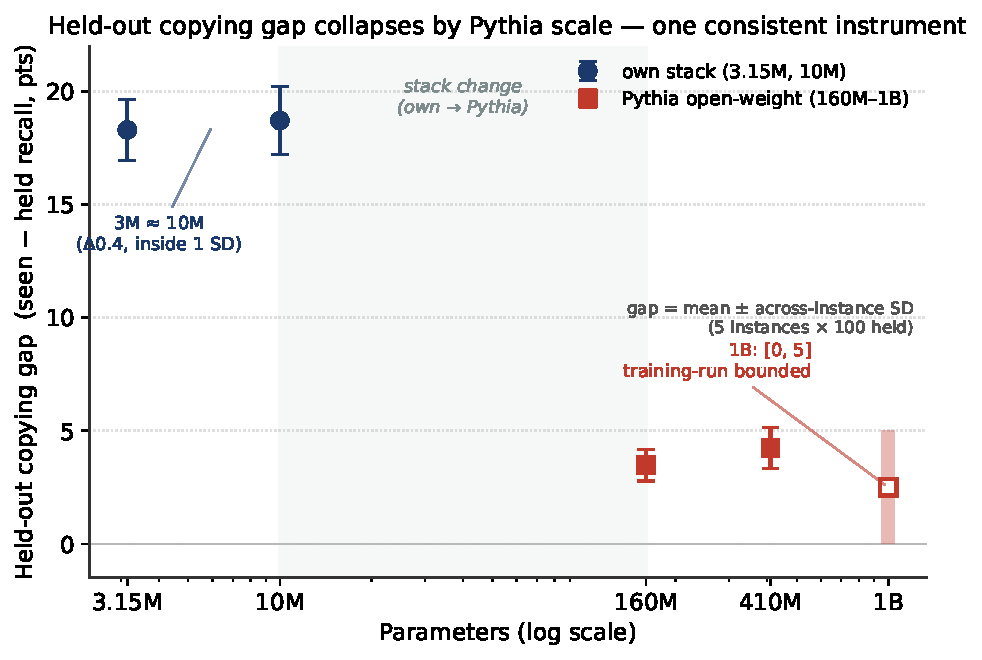
\includegraphics[width=0.85\linewidth]{fig1_gap_vs_scale.pdf}
\caption{Held-out copying gap vs.\ scale on one consistent instrument. Own-stack anchors (3.15M, 10M) sit at ${\sim}18$ pts; the tested Pythia rungs (160M, 410M) at 3.5--4.2 pts; 1B is a training-run--bounded interval $[0,5]$. The shaded band marks the own$\rightarrow$Pythia stack change --- the $x$-axis is not a pure scale axis (\S\ref{sec:limitations}).}
\label{fig:gap}
\end{figure}


\begin{figure}[t]
\centering
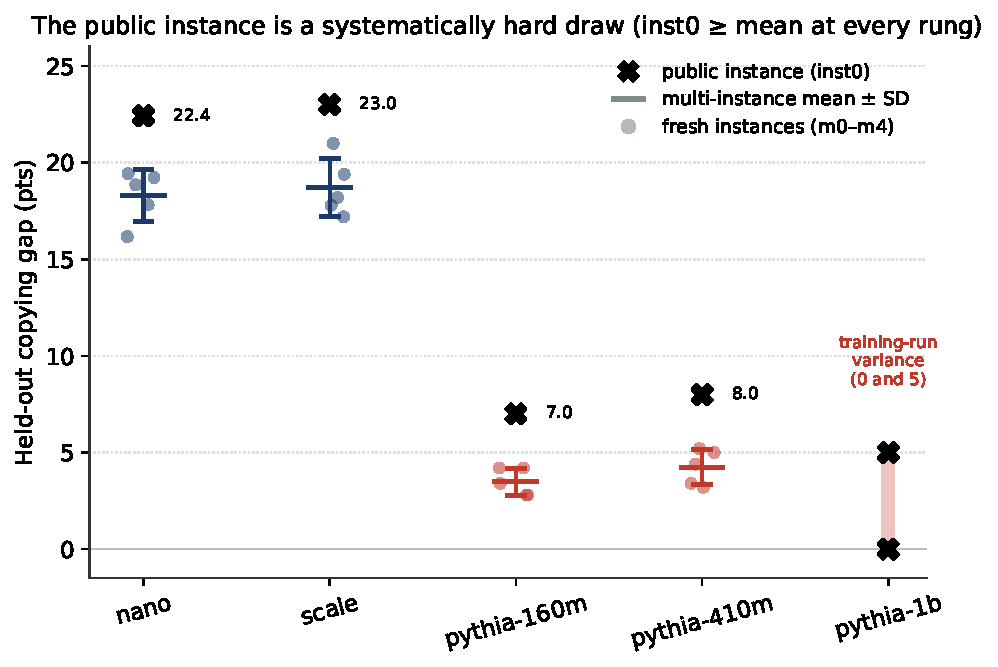
\includegraphics[width=0.85\linewidth]{fig2_instance_difficulty.pdf}
\caption{Per-rung instance difficulty. The single public instance (inst0) exceeds the five-instance mean $\pm$ SD at every rung; at 1B the two training runs (0 and 5) bracket the interval. This is why a single-instance anchor read higher than the powered mean.}
\label{fig:difficulty}
\end{figure}


\subsection{\texorpdfstring{Own-stack scale/config comparison and adaptation$\times$data interaction}{Own-stack scale/config comparison and adaptation x data interaction}}\label{sec:withinstack}

\S\ref{sec:ladder}'s ladder confounds scale with stack. Here we hold the own-stack fixed and vary adaptation and data (\S\ref{sec:withinstack}); \S\ref{sec:diversity} then varies slot diversity at fixed scale; \S\ref{sec:establish}--\S\ref{sec:lessons} interpret what is and is not established. The nano$\rightarrow$Pythia comparison confounds scale with stack. A pre-registered own-stack control at $\sim$160M (\texttt{PREREG\_ownstack\_160m.md} and factorial extensions) keeps tokenizer, architecture family, and task fixed:

 \begin{center}
\begin{tabular}{lll}
\toprule
own-stack 160M, diluted gap (clean) & 200M tokens & 3.2B tokens \\
\midrule
full FT & $\mathbf{16.9}\pm\mathbf{1.7}$ ($66.6\pm5.0$) & $\mathbf{7.0}\pm\mathbf{1.0}$ ($29.4\pm4.0$) \\
LoRA r=16 & $\mathbf{7.1}\pm\mathbf{1.2}$ ($29.6\pm3.7$) & $\mathbf{4.2}\pm\mathbf{0.9}$ ($17.7\pm3.2$) \\
\bottomrule
\end{tabular}
\end{center}

Reference: Pythia-160M (LoRA) 3.5 $\pm$ 0.7 (clean 14.7 $\pm$ 2.1). Own-stack full-FT at 200M remains large at 160M (16.9). Relative to the 3.15M / 10M anchors ($\sim$18 diluted; pretrained on \textbf{32.8M} and $\sim$\textbf{200M} tokens respectively), \textbf{no monotonic gap collapse was observed} across the evaluated configurations. Because parameter count and pretraining exposure were not fully controlled across all configurations, this is \textbf{descriptive} rather than a parameter-only causal result; the pre-registered rule still reads \textbf{stack-dominant} versus Pythia at matched size, not a smooth within-stack parameter-scale collapse. LoRA on the weak base and full FT on Chinchilla-scale data land on indistinguishable $\sim$7-point diluted gaps (seed band $\sim$$\pm$1.3 at the 200M+LoRA cell); combining both escapes yields $\mathbf{4.2}\pm\mathbf{0.9}$, near the Pythia-160M reference. We report this as a \textbf{behavioral interaction} (weak base $\times$ full-parameter adaptation). LoRA \emph{mechanism} is unidentified and not claimed here.

Across these cells the hardest low-diversity open slot (allergy under the default five-value train set) remains near-total failure in own-stack configurations and in Pythia-410M; Pythia-160M/1B show run-dependent partial rescue on that slot. Allergy is the strongest \emph{instance} of the low-diversity residual, not the definition of the phenomenon. Shared residual floor after escapes: roughly \textbf{15--18 clean points} on hard low-diversity types in both stacks (descriptive).

\emph{Table (above): own-stack 160M factorial, diluted (clean) gaps. Extends the ladder in Figure 1 --- own-stack remains elevated at 160M under full FT; escapes are adaptation$\times$data. Figure 1: \texttt{papers/figures/fig1\_gap\_vs\_scale.pdf} (stack change shaded; not a pure scale axis).}

\subsection{Slot diversity causally induces held-out copying}\label{sec:diversity}

A pre-registered type-controlled sweep (\texttt{PREREG\_slot\_diversity.md}; frozen scale-10M base, full FT; six fixed held types) varies only allergy-slot training diversity (D5 / D20 / D80) with a position control. Decision: \textbf{H-slot SUPPORTED} --- diversity effect D80-D5 = \textbf{+66.7} points held-type recall (rule $\ge$30), monotonic (0 $\rightarrow$ 24.5 $\rightarrow$ 66.7), position innocent (\textbar D20pos-D20\textbar{} = 3.1 $\le$ 5).

 \begin{center}
\begin{tabular}{lrrr}
\toprule
held type & D5 & D20 & D80 \\
\midrule
bee stings & 0 & 15 & \textbf{100} \\
ibuprofen (token-probe) & 0 & \textbf{69} & \textbf{100} \\
wool & 0 & 0 & \textbf{100} \\
strawberries & 0 & 62 & \textbf{100} \\
sulfa drugs & 0 & 0 & \textbf{0} \\
ragweed pollen & 0 & 0 & \textbf{0} \\
\bottomrule
\end{tabular}
\end{center}

\emph{Table: per-type held recall (\%) in the slot-diversity sweep (scale-10M frozen base). Residual floor: sulfa drugs and ragweed pollen remain 0 at D80 --- hardest low-diversity types, descriptive. No separate diversity figure is shipped; this table is the primary display.}

Flips are categorical per lexical type; D5 is zero across all six held types. Two types remain unsolved even at D80; token-coverage effects at the margin are \textbf{descriptive only} here, not quantified as a separate causal claim. Integrity of the frozen base checkpoint is pinned in the sweep kernel (\texttt{results\_sweep\_10m.json} provenance when run under the pinned recipe).

\subsection{What the result does and does not establish}\label{sec:establish}

Within Pythia the gap is already small at 160M with no clean monotonic trend --- and the fieldwise re-score explains why: the 160M$\rightarrow$410M flatness is a \emph{single-field} residual on the lowest-diversity open slot that scale does not reliably repair. The 3.2$\times$ own-stack step (3M$\rightarrow$10M) did not move the diluted gap (18.3$\pm$1.3 $\rightarrow$ 18.7$\pm$1.5). \S\ref{sec:withinstack} separates stack from scale at 160M: own-stack stays large under full FT; escapes are adaptation$\times$data, not parameter count alone. \S\ref{sec:diversity} shows training diversity on one slot is causally sufficient for large held-type recall gains at fixed scale. We do \textbf{not} claim generative substrate superiority (\S\ref{sec:e1}), LoRA mechanism, or open-world verification. The cross-stack ladder band is not PERSISTS (top-rung interval reaches 0); it is consistent with a small residual or none under the Pythia pipeline.

\subsection{Two distinct lessons}\label{sec:lessons}

The paper carries two takeaways that are worth keeping separate, because they are supported by different evidence and would survive independently.

\textbf{What we learned about language models.} The held-out copying gap is a \emph{pronounced small-model phenomenon}: $\sim$18 points in from-scratch models at 3--10M, essentially flat across that 3.2$\times$ scale step, and only single-digit points in the tested Pythia models at 160M and above. The fieldwise breakdown makes the phenomenon precise rather than diffuse: the gap lives \emph{entirely} in the open-vocabulary fields and is exactly zero in the closed-value fields, so what these small models fail at is specifically \textbf{copying a held-out lexical value into an open slot}, not being unfaithful in general --- and the closed-value fields are a within-task control for that claim. Measured on the actual held-out values (\S\ref{sec:ladder}, the value-level metric), the failure is not merely large but \textbf{near-total}: $\sim$80--87 points aggregate, with $\approx$0\% recall on held-out allergy values (and on held-out medications at 3M) against $\sim$100\% on seen ones --- the 18-point dialogue-level number substantially understates it. The misses are not random noise: at 10M the dominant error on held-out complaints is \textbf{substituting a memorized training complaint} (86\% of misses), while held-out allergies are omitted rather than fabricated --- memorization overriding the input in the most literal sense, and a failure mode that \emph{changes shape} with scale (nano garbles where scale substitutes). The Pythia fieldwise re-score then sharpens the picture at the other end of the ladder: the residual Pythia gap is \emph{entirely} the allergy slot --- the one open slot with only five training values --- where even 410M fails totally on the held-out value while having fully solved complaints and medications --- consistent with the low-diversity residual in \S\ref{sec:withinstack}--\S\ref{sec:diversity} (allergy is the strongest \emph{instance}, not the definition of the phenomenon). On the slot-diversity result (\S\ref{sec:diversity}), what the ladder measures is not one capability switching on but a per-slot competition between classify-and-memorize and copy, settled slot-by-slot by training diversity. What we do \textbf{not} get to say is \emph{why} it shrinks with the ladder --- the nano$\rightarrow$Pythia step changes scale together with pretraining data, tokenizer, architecture, and finetuning method (\S\ref{sec:limitations}), so the honest claim is ``the gap largely disappears by the Pythia pipeline,'' not ``parameter count removes it.'' The clean causal statements are: at this recipe, going from 3M to 10M did not move the gap; at 160M own-stack full FT the gap remains large (\S\ref{sec:withinstack}); and raising one slot's training diversity causally lifts held-type recall (\S\ref{sec:diversity}).

\textbf{What we learned about measurement.} Independently of the model result, estimating a gap like this reliably required two corrections that the data forced on us. (i) \emph{Single-instance evaluation was underpowered, and worse, biased}: the public instance is not merely noisy but \emph{systematically hard} --- its gap exceeds the multi-instance mean at every rung --- so a fixed public instance can skew an effect size even when it is content-addressed and reproducible. (ii) \emph{The precision floor moves with the regime}: in the high-gap regime the dominant uncertainty is across evaluation instances, but by 1B the gap is small and the dominant uncertainty becomes the \emph{training run} (two fixed-seed retrains split 5/0), so the right replication unit changes from eval-instance to training-seed. Both lessons are prescriptive for anyone measuring faithfulness gaps in small models and hold regardless of how the scale-vs-stack question is eventually resolved. Separately, our primary metric is exact string match: it has not been validated against human-accepted equivalence, so reported gaps may overstate failure relative to a soft/human rubric (\S\ref{sec:e1}, \S\ref{sec:limitations}).

\section{Limitations}\label{sec:limitations}

\begin{itemize}
\item
  \textbf{Scale vs.~stack confound (primary).} The nano$\rightarrow$Pythia comparison changes parameter count \emph{and} at least four other variables simultaneously, each a plausible alternative cause of the reduction: (i) \textbf{pretraining data quantity} ($\sim$200M own-stack tokens vs. Pythia's $\sim$300B --- a $\sim$1500$\times$ difference; the own-stack is roughly compute-optimal for its size per Hoffmann et al.~(2022), whereas Pythia is heavily over-trained), (ii) \textbf{tokenizer} (4098-vocab BPE vs.~$\sim$50k; larger vocabularies fragment field values like ``ibuprofen'' into fewer sub-tokens, which could itself change copy success), (iii) \textbf{architecture family}, and (iv) \textbf{finetuning method} (own-stack full fine-tune vs.~Pythia LoRA r=16 --- a behavioral adaptation-regime difference; mechanism unidentified). We therefore claim only that the gap is much smaller under the Pythia \emph{pipeline}, not that scale per se removes it. The within-stack / factorial separation of scale from that stack bundle is reported in \S\ref{sec:withinstack}.
\item
  \textbf{Transition point unobserved.} The gap drops somewhere between own-stack 10M (18.7) and Pythia-160M (3.5), but those endpoints are on different stacks; within Pythia the gap is already low at 160M with no monotonic trend, so ``by Pythia scale'' is safe while ``as models scale up'' is not yet supported.
\item
  \textbf{1B point estimate.} Bounded, not identified, by training nondeterminism (\S\ref{sec:nondet}).
\item
  \textbf{Exact-match construct (explicit).} Primary science metrics are exact string match. Normalize-then-match rescues 0/486 M0 exact failures (E3 auto), but exact-match has \textbf{not} been validated against human-accepted equivalence; gaps may overstate failure vs a soft/human rubric (\S\ref{sec:e1}). Discontinuous metrics can also exaggerate transitions (Schaeffer et al. 2023); we report across-instance SD and, at 1B, a training-run interval.
\item
  \textbf{Gap-definition subtleties (conservative direction).} The seen/held split is at the dialogue level, so the held bucket mixes in seen field-values (a ``held'' dialogue draws a held-out value only per-field-probabilistically); and recalls are computed over parsed dialogues only, where at the nano rung the held split parses slightly less often than the seen split. Both push the \emph{measured} gap toward zero, so reported gaps (aggregate and per-field) are conservative lower bounds on the pure held-out-value effect; neither biases the cross-model comparison, which uses the identical instrument.
\item
  \textbf{Single task and single scale family.} One synthetic clinical-summarization task; one scaling family. Generality across domains and families is untested here.
\item
  \textbf{Anchor precision (resolved).} The 3M/10M anchors were re-scored on the same multi-instance instrument as the rest of the ladder (18.3$\pm$1.3, 18.7$\pm$1.5); the whole ladder now shares one instrument, and the anchor gaps carry across-instance SD like the Pythia rungs.
\item
  \textbf{Out of scope (gated).} LoRA mechanism identification, fabric/product work, and further residual continua are out of scope here (\texttt{papers/EMPIRICAL\_FOUNDATION.md}). No mechanism, product, or open-world verification claims are advanced.
\end{itemize}

\section{Conclusion}\label{sec:conclusion}

A severe held-out copying gap in sub-10M models --- failure to copy held-out lexical values into open slots, with closed-value fields a zero-gap control --- is much smaller under the tested Pythia pipeline. Across the evaluated own-stack configurations, the diluted gap did not decrease monotonically with parameter count; parameter count was not isolated from total pretraining exposure, so this is descriptive rather than a parameter-only scale law. Adaptation$\times$data accounts for most of the escape to Pythia-like levels. Slot training diversity causally raises held-type recall (+66.7). On a pre-registered utility, \textbf{M1} exceeds the best evaluated generative reference under frozen $U$ (\S\ref{sec:e1}) --- recorded as a kill-gate result, not a product pitch. Exact-match remains an explicit construct limitation (automated normalize + agent-applied rubric audit; dual-clinician validation unperformed). The measurement story is inseparable from the result: single-instance evaluation was under-powered, and at the top of the ladder training nondeterminism sets the precision floor. The contribution is a careful empirical account of when small LMs fail held-out emission, with limitations kept visible rather than explained away.

\phantomsection

\paragraph{Reproducibility.}
All eval instances, recipes, scorers, per-run result files, and library versions are
content-addressed and archived in the public repository
(\url{https://github.com/wwk5q8z6kk-bit/nano-lm}); every number regenerates from
committed artifacts. Bibliographic keys live in \texttt{refs.bib}.

\nocite{*}
\bibliographystyle{plainnat}
\bibliography{refs}

\end{document}

